\chapter{Discrete-Time Linear Autoregressive Poisson Models}
\label{chap:four}

This short chapter builds on the network Hawkes model introduced in
the last. We introduce linear autoregressive Poisson models --- the discrete time analogue of the Hawkes process --- and we derive efficient Gibbs sampling
and stochastic variational inference algorithms, leveraging the sample
superposition principle as before. This chapter marks the transition
from continuous models to the discrete time models that occupy this
and subsequent chapters. As we will see, these discrete time formulations
are in some ways easier to work with. We can easily extend them to non-Poisson
spike count models, and we can interface with the diverse array of
probabilistic matrix decomposition models. However, the discrete
nature of spike counts still poses some serious inferential hurdles,
which this thesis aims to overcome.

In addition to briding from continuous to discrete, this chapter also
addresses issues of computational complexity. The complexity of our Hawkes process
inference algorithm scaled, in the worst case, quadratically with the
number of spikes, since we had to sample a ``parent'' for each spike.
By designing block parallel Gibbs updates, we were able
to obtain linear complexity. However, when the firing rates are high,
this is still the bottleneck of our algorithm. Here we show that in
some regimes we can reduce this complexity to be independent
of the number of spikes by adopting a discrete time approach.
Moreover, we derive efficient \emph{stochastic} variational inference
algorithms that work with subsets of time bins in each iteration
and thereby scale to massive datasets.


\section{Discrete Time Linear Autoregressive Poisson Models}

The fundamental limitation of the previously developed continuous time
models is that the number of values that the auxiliary
variable~$\omega_m$ can take grows with the number of events which
occurred before time~$s_{m}$. For datasets with high rates of
activity, this can quickly become the limiting factor of the inference
algorithm.  At the same time, it is often reasonable to assume that
events do not interact on time scales faster that~$\Delta t$. This
motivates a discrete time formulation in which we bin events in bins
of width~$\Delta t$ and ignore potential interactions between events
in the same bin. Then the rate becomes,
\begin{align}
\label{eq:disc_hawkes_rate}
\lambda_{t,n} &= \lambda_n^{(0)} +
\sum_{n' = 1}^N \sum_{d=1}^{D} s_{t-d,n'} \cdot h_{n' \to n}[d], \\
s_{t,n} &\sim \distPoisson(\lambda_{t,n} \cdot \Delta t),
\end{align}
where~$s_{t,n}$ is the number of spikes fired by neuron~$n$ in the
$t$-th time bin and~${h_{n' \to n}[d]}$ is an impulse response
function describing the influence that events on neuron~$n'$ have on
the rate of process~$n$ at discrete time lag~${d}$. As we will show,
under this formulation the auxiliary variables only assume a fixed set
of values independent of the rate.

As before, we introduce a network model as a prior distribution over
the impulse response weights. Following the approach of the previous
chapter, we decompose the impulse response function into the product
of a binary variable that specifies whether or not a connection
exists, a scalar weight that specifies the strength of the interaction
if present, and a probability mass function that specifies the time
course of interaction:
\begin{align*}
  h_{n \to n'}[d]
  &= a_{n \to n'} \cdot w_{n \to n'} \cdot \hbar[d; \, \btheta_{n \to n'}] 
\end{align*}
for~${d \in\{1,\ldots,D\}}$.  
The function~${\hbar[d]: \{1, \ldots, D\} \to
  [0,1]}$ is now a probability mass function, which we model as a convex
combination of normalized basis functions,~$\bphi_b$,
\begin{align*}
  \hbar[d; \, \btheta_{n \to n'}]
  &\triangleq \sum_{b=1}^B \theta_{n \to n'}^{(b)} \cdot \phi_b[d], \\
  \sum_{d=1}^D \phi_b[d] \cdot \Delta t  &= 1, \\
  \sum_{b=1}^B \theta_{n \to n'}^{(b)} &= 1.
\end{align*}
We enforce the latter constraint with a Dirichlet
prior~${\btheta_{n \to n'} \sim \distDirichlet(\bgamma)}$.
The basis functions are typically taken to be normalized Gaussian bumps or
rectified cosine functions spaced over the interval~${1,\ldots,D}$.

Plugging this impulse response model
into~Eq.~\ref{eq:disc_hawkes_rate} yields,
\begin{align*}
  \lambda_{t,n'} &=
  \lambda_{n'}^{(0)} +
  \sum_{n = 1}^N  \sum_{b=1}^B a_{n \to n'} \cdot w_{n \to n'} \cdot 
  \theta_{n \to n'}^{(b)} \sum_{t'=1}^{t-1} s_{t',n} \cdot \phi_b[d] \\
  &=
  \lambda_{n'}^{(0)} +
  \sum_{n' = 1}^N  \sum_{b=1}^B a_{n \to n'} \cdot w_{n \to n'} \cdot
  \theta_{n \to n'}^{(b)} \cdot  \widehat{s}_{t,n,b},
\end{align*}
where
\begin{align*}
  \widehat{s}_{t,n,b} &\triangleq \left(\bs_n \ast \bphi_b\right)[t],
\end{align*}
is the discrete convolution of the~$n$-th spike train with
the~$b$-th basis function evaluated at the~$t$-th time bin.
Since both the spike trains and the basis functions are given,
these can be precomputed.


\section{Inference with Gibbs Sampling}

As before, we begin by introducing auxiliary parent variables for each
entry~$s_{t,n}$.  By the superposition theorem for Poisson processes,
each event can be attributed to either the background rate or one of
the impulse responses.

Let~${\omega_{t,n'}^{(n,b)} \in \{0,\ldots, s_{t,n'}\}}$ denote how
many of the events that occurred in the~$t$-th time bin on the~$n'$-th
neuron are attributed to the~$b$-th basis function of the~$n$-th
neuron.  Similarly, let~${\omega_{t,n'}^{(0)}}$ denote the number of
events attributed to the background process. We combine these
auxiliary variables into vectors,~${\bomega_{t,n'}\triangleq
  \left[\omega_{t,n'}^{(0)}, \omega_{t,n'}^{(1,1)}, \ldots,
    \omega_{t,n'}^{(N,B)} \right]}$.

Due to the Poisson superposition principle, these parent variables are
conditionally multinomial distributed.  For time~$t$ and neuron~$n'$,
we resample
\begin{align*}
\bomega_{t,n'} &\sim \distMultinomial \left(s_{t,n'}, \bu_{t,n'} \right) & 
u_{t,n'}^{(0)} &= \frac{\lambda_{n'}^{(0)}[t]}{\lambda_{n'}[t]}, &
u_{t,n'}^{(n,b)} &= \frac{\hat{s}_{t,n,b} \cdot a_{n \to n'} \cdot w_{n \to n'} \cdot \theta_{n \to n'}^{(b)}}{\lambda_{n'}[t]}\, .
\end{align*}
Given this attribution, the likelihood factorizes into a product of
Poisson distributions,
\begin{multline*}
  p(\bomega \given \blambda) =
  \left[\prod_{t=1}^T \prod_{n'=1}^N \distPoisson(\omega_{t,n'}^{(0)} \given \lambda_{n'}^{(0)} \Delta t)\right]  \\
  \times
  \left[ \prod_{t=1}^T \prod_{n=1}^N \prod_{n'=1}^N \prod_{b=1}^B
    \distPoisson(\omega_{t,n'}^{(n,b)} \given
    \hat{s}_{t,n,b} \cdot a_{n \to n'} \cdot w_{n \to n'} \cdot \theta_{n\to n'}^{(b)} \cdot \Delta t)\right].
\end{multline*}

\paragraph{Gibbs sampling the background rates.}
We use conjugate priors for the constant background rates, weights,
and impulse responses.  For the constant background rates we have,
${\lambda_{n'}^{(0)} \sim\distGamma(\alpha_\lambda, \beta_\lambda)}$,
which results in the conditional distribution
\begin{align*}
\lambda_{n'}^{(0)} \given \{\omega_{t,n'}^{(0)}\} &\sim
\distGamma(\alpha_\lambda^{(n)}, \beta_\lambda^{(n)}), \\
\alpha_\lambda^{(n)} &= \alpha_\lambda + \sum_{t=1}^T \omega_{t,n'}^{(0)}, \\
\beta_\lambda^{(n)} &= \beta_\lambda + T \Delta t\,.
\end{align*}

\paragraph{Gibbs sampling impulse responses.}
The likelihood of the impulse responses,~$\btheta_{n \to n'}$ is
proportional to a Dirichlet distribution.  Combined with
a~$\text{Dirichlet}(\bgamma)$ prior this yields
\begin{align*}
  \btheta_{n \to n'} \given \{\omega_{t,n}^{(n',b)}\}, \bgamma
  &\sim \distDirichlet\left( \bgamma_{n \to n'} \right), \\
  \gamma_{n \to n'}^{(b)} &=  \gamma_b + \sum_{t=1}^T \omega_{t,n'}^{(n, b)}\,.
\end{align*}

\paragraph{Gibbs sampling the weighted adjacency matrix.}
As before, the weights are conjugate with a gamma
prior,~$\distGamma(\kappa, \nu_{n \to n'})$, where the scale is presumed to
be given by the network prior.  Given the adjacency matrix~$\bA$
and the auxiliary parent variables, the conditional distribution is,
\begin{align*}
  w_{n \to n'} \given a_{n \to n'}\!=\!1
  &\sim \distGamma(\widetilde{\kappa}^{(n,n')}, \widetilde{\nu}^{(n,n')}), \\
  \widetilde{\kappa}^{(n,n')} &= \kappa + \sum_{t=1}^T \sum_{b=1}^B \omega_{t,n'}^{(n,b)}, \\
  \widetilde{\nu}^{(n,n')} &= \nu_{n \to n'} +  \sum_{t=1}^T s_{t,n}.
\end{align*}
As in the previous chapter, in order to resample~$\bA$, we iterate over
each entry and sample from the marginal distribution after integrating
out the parents. We assume the parameters of the network prior can be
sampled efficiently --- a reasonable assumption for many random network
models.

The continuous time representation introduces a latent ``parent''
variable for each event in the dataset, and the parent can be any one
of the events that occurred in the preceding window of influence. Call
the number of potential parents~$M$. The discrete time representation
has a multinomial random variable for each time bin that contains at least one
event, and the support of this multinomial is always a fixed
size,~${NB+1}$.  When the rate of events is high, $NB+1 \ll M$,
allowing for dramatic improvements in efficiency in the discrete case.

% Discrete vs continuous figure
\begin{figure}[t]
  \centering
  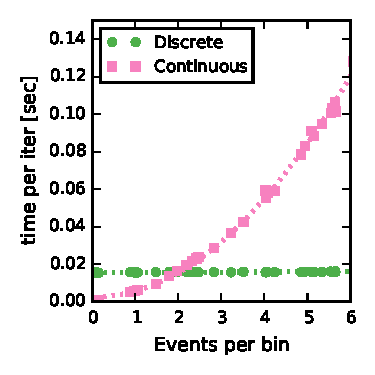
\includegraphics[width=2.5in]{figures/ch4/discrete_cont_comparison}
  \caption[Runtime comparison of continuous and discrete time Hawkes models]{
    Comparison of run time per Gibbs sweep for the discrete and continuous network Hawkes formulations. Best fit lines added.}
  \label{fig:disc_vs_cont}
\end{figure}


Figure~\ref{fig:disc_vs_cont} shows the time per full Gibbs sweep as a
function of the number of events per discrete time bin for the
discrete and continuous formulations. The discrete formulation incurs
a constant penalty whereas the continuous formulation quickly grows
with the event rate. For low rates, the continuous formulation can be
advantageous, but the discrete model is vastly superior in many
realistic settings. For example, in Chapter~\ref{chap:three} we worked with
trades on the S\&P100, which occur tens or hundreds of times per
second for each stock. Since the complexity of our continuous time algorithm grew
with the number of events, we had to down-sample the data to consider only
the times when stock prices changed significantly. However, we
were also looking for interactions on time scales of one minute,
very large compared to the rate of trades. Thus, it is
reasonable to consider a discrete time model in which the number of
trades is counted in, say, $1$sec bins instead. The discrete time
methods of this chapter would allow us to work directly with this type of
trade-level activity and still scale to days or weeks of data.

\section{Stochastic Variational Inference}
The discrete time formulation offers advantageous complexity compared
to the continuous analogue, but in order to maintain the invariance of
the posterior distribution, we must still work with the entire set of
parents each iteration. In many cases, a subset, or ``mini-batch,'' of
time bins can provide substantial information about the global
parameters of the model, and rapid progress can be made by iterating
quickly over subsets of the data. This motivates our derivation of a
stochastic variational inference (SVI) algorithm for this discrete
time model.

Variational methods optimize a lower bound on the marginal likelihood
by minimizing the KL-divergence between a tractable approximating
distribution and the true posterior. Since the local parents
variables,~$\bomega$, are conditionally independent given the global
parameters~($\bA$,~$\bW$,~$\btheta$,~etc.), our variational approach will
easily extend to the stochastic setting in which we compute unbiased
estimates of the gradient of the variational objective using
mini-batches of data.

The primary impediment to deriving a variational approximation is the
nonconjugacy of the spike-and-slab prior on the weights.  To overcome
this, we approximate the spike-and-slab prior with a mixture of gamma
distributions, as has previously explored by~\citet{Grabska-2013}:
\begin{align*}
  p(\bA, \bW \given \{\bz_n\}, \bvartheta)
  &= \prod_{n,n'} p(a_{n \to n'} \given \bz_n, \bz_{n'}, \bvartheta) \, p(w_{n \to n'} \given a_{n \to n'}, \bz_n, \bz_{n'}, \bvartheta) \\
  p(a_{n \to n'} \given \bz_n, \bz_{n'}, \bvartheta) &= \distBernoulli(a_{n \to n'} \given \rho_{n \to n'}), \\
  p(w_{n \to n'} \given a_{n \to n'}, \bz_n, \bz_{n'}, \bvartheta)
  &=
  \begin{cases} 
    \distGamma(w_{n \to n'} \given \kappa, \nu_{n \to n'}, a_{n \to n'} =1), \\
    \distGamma(w_{n \to n'} \given \kappa_0, \nu_0, a_{n \to n'} =0),
  \end{cases}
\end{align*}
where, as before,~$\rho_{n \to n'}$ and~$\nu_{n \to n'}$ are functions
of the latent variables,~$\bz_n$ and~$\bz_{n'}$, and the
parameters~$\bvartheta$.  We have approximated the ``spike'' in the
spike-and-slab model with a gamma distribution parameterized
by~$\kappa_0$ and~$\nu_0$.  As~$\kappa_0 \to 0$ and~$\nu_0\to \infty$,
the gamma distribution approaches a spike at zero.

This approximate probabilistic model is now amenable to mean field
variational inference. We use a fully-factorized variational
approximation, with the exception of a joint factor for each
connection,~${(a_{n\to n'},w_{n \to n'})}$.
\begin{align*}
  q(a_{n \to n'}) &= \distBernoulli(a_{n \to n'} \given \widetilde{p}_{n \to n'}), \\
  q(w_{n \to n'} \given a_{n \to n'}) &=
  \begin{cases} 
    \distGamma(w_{n \to n'} \given \widetilde{\kappa}_1^{(n, n')}, \widetilde{\nu}_1^{(n,n')}, a_{n \to n'} =1), \\
    \distGamma(w_{n \to n'} \given \widetilde{\kappa}_0^{(n, n')}, \widetilde{\nu}_0^{(n, n')}, a_{n \to n'} =0)\,.
  \end{cases}
\end{align*}
Since the model is fully conjugate, the factors are easily derived.

% Parents
\paragraph{Variational updates for parent variables,~$q(\bomega_{t, n'})$} 
For the parent variables, the variational updates are
\begin{align*}
q(\bomega_{t,n'}) &= \distMultinomial(\bomega_{t, n'} \given s_{t,n'}, \widetilde{\bu}_{t,n'}), \\
\widetilde{u}_{t,n'}^{(0)} &= \frac{1}{Z} \exp\left\{\mathbb{E}_{\blambda}[\ln \lambda_{n'}^{(0)}]\right\}, \\
\widetilde{u}_{t,n'}^{(n,b)} &= \frac{1}{Z} \hat{s}_{t,n,b} \exp\left\{\mathbb{E}_{\btheta} [\ln \theta_{n \to n'}^{(b)}] + \mathbb{E}_W[\ln w_{n \to n'}]\right\},
\end{align*}
where~$Z$ is the normalization constant.

% Background rates
\paragraph{Variational updates for background rates,~$q(\lambda_n^{(0)})$}
The variational form parameters of the gamma distribution over
background rates are
\begin{align*}
q(\lambda_n^{(0)}) &= \distGamma(\lambda_n^{(0)} \given \widetilde{\alpha}_{\lambda}^{(n)}, \widetilde{\beta}_{\lambda}^{(n)}),  \\
\widetilde{\alpha}_{\lambda}^{(n)} &= \alpha_\lambda + \sum_{t=1}^T \mathbb{E}_{\bomega}\left[ \omega_{t,n}^{(0)}\right], \\
\widetilde{\beta}_{\lambda}^{(n)} &= \beta_\lambda + T \Delta t\,.
\end{align*}


% Impulse response parameters
\paragraph{Variational approximation for impulse response parameters,~$q(\btheta_{n \to n'})$}
With the conjugate prior formulation the variational parameter updates
for the Dirichlet distributed impulse response parameters are
\begin{align*}
q(\btheta_{n \to n'}) &= \distDirichlet(\bn_{n \to n'} \given \widetilde{\bgamma}^{(n,n')}), \\
\widetilde{\gamma}_b^{(n,n')} &= \gamma_{b} + \sum_{t=1}^T \mathbb{E}_{\bomega}\left[\omega_{t,n'}^{(n,b)}\right]\,.
\end{align*}

% Weights and adjacent matrix
\paragraph{Variational approximation for the weighted adjacency matrix.}
The primary motivation for adopting a weakly sparse mixture of gamma
distributions is to derive an efficient variational inference
algorithm.  The mixture-of-gammas prior is conjugate with the Poisson
observations, and hence the variational distribution is also a mixture
of gammas:
\begin{align*}
  q(w_{n \to n'} \given a_{n \to n'}=1)
  &= \distGamma(w_{n \to n'} \given
  \widetilde{\kappa}^{(n,n')}_1,
  \widetilde{\nu}^{(n,n')}_1) \\
  \widetilde{\kappa}^{(k,k')}_1
  &= \kappa + \sum_{t=1}^T \sum_{b=1}^B \mathbb{E}_{\bomega}\left[\omega_{t,n'}^{(n,b)}\right] \\
  \widetilde{\nu}^{(n,n')}_1
  &= \nu_{n \to n'} + \sum_{t=1}^T s_{t,n}\,,
\end{align*}
and likewise for the ``spike'' factor,
\begin{align*}
  q(w_{n \to n'} \given a_{n \to n'}=0)
  &= \distGamma(w_{n \to n'} \given
  \widetilde{\kappa}^{(n,n')}_0,
  \widetilde{\nu}^{(n,n')}_0) \\
  \widetilde{\kappa}^{(k,k')}_0
  &= \kappa_0 + \sum_{t=1}^T \sum_{b=1}^B \mathbb{E}_{\bomega}\left[\omega_{t,n'}^{(n,b)}\right] \\
  \widetilde{\nu}^{(n,n')}_0
  &= \nu_0 + \sum_{t=1}^T s_{t,n}\,,
\end{align*}

% Adjacency matrix
This leaves us with~$q(a_{n \to n'})$, which is Bernoulli distributed
with parameter~$\widetilde{p}_{n \to n'}$. The optimal parameter is given by,
\begin{multline*}
  \frac{\widetilde{p}_{n \to n'}}{1-\widetilde{p}_{n \to n'}} =  
  \frac{\exp\{\mathbb{E} [\ln \rho_{n \to n'}] \} }{\exp\{\mathbb{E}[\ln (1-\rho_{n \to n'})] \}} \times \\
  \frac{ (\exp\{\mathbb{E} [\ln \nu_{n \to n'}] \})^{\kappa} }{ \Gamma(\kappa)} \times 
  \frac{\Gamma(\widetilde{\kappa}^{(n,n')}_1)}{ (\widetilde{\nu}^{(n,n')}_1)^{\widetilde{\kappa}^{(n,n')}_1} } \times
  \frac{\Gamma(\kappa_0)}{ (\nu_0)^{\kappa_0} } \times
  \frac{(\widetilde{\nu}^{(n,n')}_0)^{\widetilde{\kappa}^{(n,n')}_0}}{ \Gamma(\widetilde{\kappa}^{(n,n')}_0)}\,.
\end{multline*}

% network model
As with Gibbs sampling, we assume a variational approximation for the
network model can be derived, and provide access to the necessary
expectations,~$\mathbb{E}[\ln \rho_{n \to n'}]$,
$\mathbb{E}[\ln(1-\rho_{n \to n'})]$,~$\mathbb{E}[\nu_{n \to n'}]$ and~$\mathbb{E}[\ln \nu_{n \to n'}]$.

As aforementioned, the time bin are conditionally independent given
the network weights and the adjacency matrix -- a common pattern
exploited by stochastic variational inference (SVI) algorithms
\cite{Hoffman-2013}.  These methods optimize the variational objective
using stochastic gradient methods that work with mini-batches of data.
Often, a mini-batch of data can provide valuable information about the
global parameters, in our case the network and background rates.
Quickly iterating over these global parameters allows us to reach good
modes of the posterior distribution in a fraction of the time that
standard variational Bayes and Gibbs sampling require, since those
methods must process the entire dataset before making an update.  SVI
does require some tuning, however. In particular, we must set a
mini-batch size and a step size schedule.  In this work, we fix the
mini-batch size to~${T_{\mathsf{mb}}=1024}$ and set the step size at
iteration~$i$ to~${(i+1)^{-0.5}}$.  These parameters may be tuned with
general purpose hyperparameter optimization techniques
\cite{Snoek-2012}.

%% Synthetic Results 
\section{Synthetic Results}

% Predictive log likelihood vs run time (Short dataset)
\begin{figure}[t!]
  \begin{center}
    % Short dataset
    \begin{subfigure}[b]{0.48\linewidth}
      \caption{Short dataset: $T=10^4$}
      \centering
      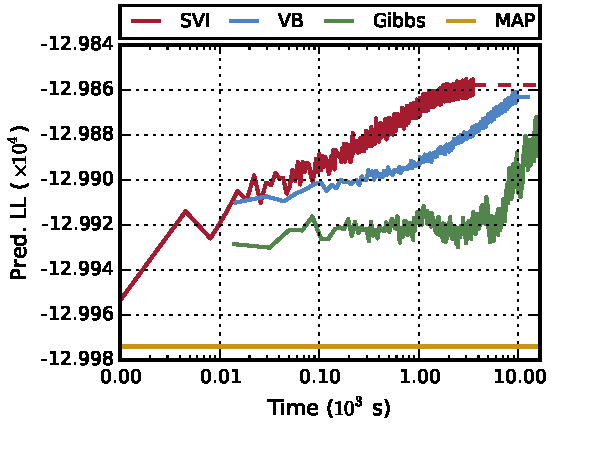
\includegraphics[width=2.625in]{figures/ch4/figure2a.pdf} 
      \label{fig:synth_pll_short}
    \end{subfigure}
    ~
    % Longer dataset
    \begin{subfigure}[b]{0.48\linewidth}
      \caption{Long dataset: $T=10^5$}
      \centering
      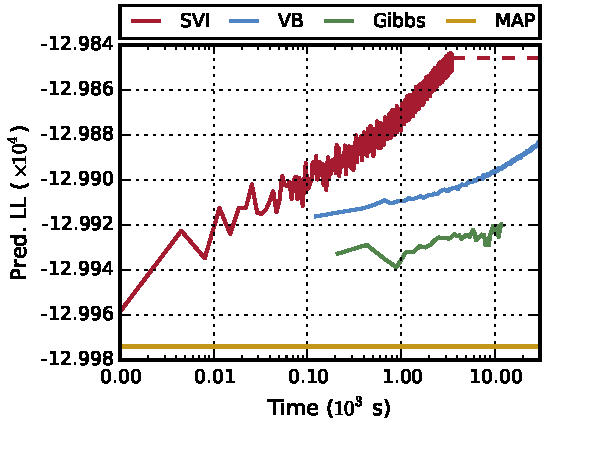
\includegraphics[width=2.625in]{figures/ch4/figure2b.pdf} 
      \label{fig:synth_pll_long}
    \end{subfigure}
    %
    \caption[Predictive log likelihood versus wall clock time]{
      Predictive log likelihood versus wall clock time for three
      Bayesian inference algorithms on a dataset of~$N=50$ neurons
      and~$T=10^4$ and~$T=10^5$ time bins on the left and right,
      respectively.}
    \label{fig:synth_pll}
  \end{center}
\end{figure}


We assess the performance of the proposed inference algorithms on a
synthetic dataset generated by a strongly sparse Hawkes process
with~${N=50}$ neurons.  We used a stochastic block model network
prior with~${K=5}$ clusters, each consisting of ten densely connected
processes~(${p_{k\to k}=0.4}$), with sparse connections to processes
in other clusters~(${p_{l\to k'}=0.01}$).  All weights share the same
scale of~$\nu=5.0$, though this information is not provided \emph{a
  priori}.  We simulate~${T=10^5}$ time bins in steps of size~${\Delta
  t=1}$.  The neurons have an mean background rate of~$1.0$ event
per time bin and, due to the network interactions, the average total
rate of the processes is~$16.7 \pm 12.0$ events per bin.  Referring to
Figure~\ref{fig:disc_vs_cont}, this is a regime that favors the
discrete model.  We initialized by performing MAP estimation on the
first~$T_{\mathsf{init}}=10^4$.  Then we trained the model using Gibbs
sampling, batch variational Bayesian inference (VB), and stochastic
variational inference (SVI)

We trained the models on only the first~$10^4$ time bins, the same
that were used for initialization.  We evaluated the algorithms in
terms of their predictive log likelihood on a held-out dataset of
length~$T_{\mathsf{test}}=10^3$.  Figure~\ref{fig:synth_pll_short}
shows the results as a function of wall-clock time.  We find that SVI
obtains competitive predictive log likelihood in a matter of minutes.
Batch VB and Gibbs converge at a considerably slower rate, though they
eventually match the SVI predictive likelihood after hours of
computation.  The MAP estimate, even with cross validated
regularization, underperforms the other competing algorithms.

This trend is amplified when we consider the entire training set of
size~$T=10^5$.  Figure~\ref{fig:synth_pll_long} illustrates the power
of SVI in handling these large time datasets.  Considerable
information about the global parameters (e.g., the network) can be
gained from just a mini-batch of time points.  Hence, we can make
rapid improvements in predictive log likelihood very quickly.  By
contrast, each step of the Gibbs and batch VB algorithms is
approximately $10$ times slower, and even after computing sufficient
statistics over the entire dataset, the algorithm is only able to make
limited progress per iteration.

% Some results on a connectomics dataset
\section{Connectomics Results}

% Connectomics results
\begin{figure}[t!]
  \begin{center}
    % a. the data
    \begin{subfigure}[b]{0.32\linewidth}
      \caption{}
      \centering
      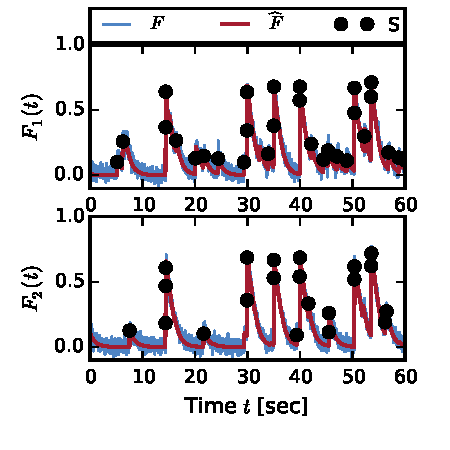
\includegraphics[width=\textwidth]{figures/ch4/figure3a.pdf} 
      \label{fig:connectomics_data}
    \end{subfigure}
    % b. True network with block structure
    ~
    % c. ROC
    \begin{subfigure}[b]{0.32\linewidth}
      \caption{}
      \centering
      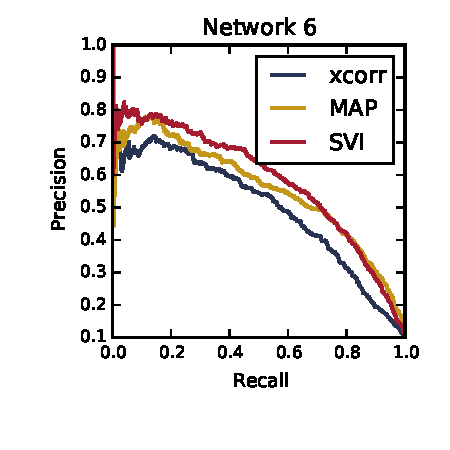
\includegraphics[width=\textwidth]{figures/ch4/figure3d.pdf} 
      \label{fig:connectomics_prc}
    \end{subfigure}
    ~
    % d. Precision Recall
    \begin{subfigure}[b]{0.32\linewidth}
      \caption{}
      \centering
      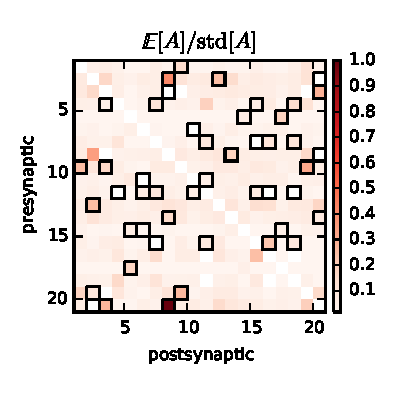
\includegraphics[width=\textwidth]{figures/ch4/chalearn_confidence.pdf} 
      \label{fig:connectomics_zscore}
    \end{subfigure}
    % Main caption
    \caption[Discrete time Hawkes process applied to connectomics challenge]{
      Application of the network Hawkes model to a connectomics challenge.
      \textbf{(a)} The data is in the form of a calcium fluorescence trace, which we preprocess to extract neural spike times.
      \textbf{(b)} We measure performance on a link prediction task using a precision-recall curve and find that the posterior estimates of SVI provide the best estimates on some networks. In addition to an estimate of the connection probability and weight, SVI provides an estimate of the posterior uncertainty.
      \textbf{(c)} Inferred $\mathbb{E}_q[\bA] / \text{std}_q[\bA]$ for the first 20 neurons. True connections are outlined in black.}
    \label{fig:connectomics}
  \end{center}
\end{figure}

We tested these inference algorithms on the data from the Chalearn
neural connectomics
challenge\footnote{\url{http://connectomics.chalearn.org}}
\cite{Stetter-2012}.  The data consist of calcium fluorescence
traces,~$\bF$, from six networks of~$N=100$ neurons each. We use ten
minutes of data at 50Hz sampling frequency to yield~$T=3\times 10^6$
entries in~$\bS$.  In this case, the networks are purely excitatory,
and each action potential, or spike, increases the probability of the
downstream neurons firing as a result.  This matches the underlying
intuition of the Hawkes process model, making it a natural choice.

In order to apply the Hawkes model, we first convert the fluorescence
traces into a spike count matrix using OOPSI, a Bayesian inference
algorithm based on a model of calcium fluorescence
\cite{Vogelstein-2010}.  The output is a filtered fluorescence
trace,~$\widehat{\bF}$, and a probability of spike for each time bin.
We threshold this at probability~$0.7$ to get a~$T\times N$ binary
spike matrix,~$\bS$.  This preprocessing is shown in
Figure~\ref{fig:connectomics_data}.

Figure~\ref{fig:connectomics_prc} shows the precision-recall curve we
used to evaluate the algorithms' performance on network recovery. As a
baseline, we compare against simple thresholding of the cross
correlation matrix. On Network 6, SVI offers the best network
inference. Table~\ref{tab:chalearn} shows the results on the other
five networks using the same model parameters. On 4/5 of these
networks, the Bayesian methods offer the best performance.

Figure~\ref{fig:connectomics_zscore} illustrates one of the main
advantages of the fully Bayesian inference algorithm -- calibrated
estimates of posterior uncertainty. Here we show the SVI algorithm's
estimate of the posterior mean of~$\bA$ normalized by the posterior
standard deviation for a subset of 20 neurons from Network 6. We also
outline the true connections to show that the most confident
predictions are more likely to correspond to true connections. Such
estimates of the posterior uncertainty are not available with standard
heuristic methods or point estimates.

% A fancy table with results for each of the networks
\begin{table}
  \centering
  \resizebox{\textwidth}{!}{%
    \begin{tabular}{ c||c|c||c|c||c|c||c|c||c|c }
      %\hline
      %\multirow{3}{*} \textbf{Algorithm} 
      & \multicolumn{2}{c||}{Network 1}
      & \multicolumn{2}{c||}{Network 2}
      & \multicolumn{2}{c||}{Network 3}
      & \multicolumn{2}{c||}{Network 4}
      & \multicolumn{2}{c}{Network 5} \\
      \cline{2-11}
      Algorithm
      & ROC & PRC
      & ROC & PRC
      & ROC & PRC
      & ROC & PRC
      & ROC & PRC \\
      %\hhline{=#=|=#=|=#=|=#=|=#=|=}
      \hline
      xcorr & $0.596$ & $0.139$ & $0.591$ & $0.133$ & $\bf{0.701}$ & $\bf{0.198}$ & $0.745$ & $0.296$ & $0.798$ & $0.359$  \\
      \hline
      MAP & $0.607$ & $0.174$ & $\bf{0.619}$ & $\bf{0.143}$ & $0.698$ & $0.178$ & $\bf{0.790}$ & $0.334$ & $\bf{0.859}$ & $0.408$ \\
      \hline
      SVI  & $\bf{0.649}$ & $\bf{0.184}$ & $0.605$ & $0.141$  & $0.673$ & $0.176$ & $0.774$ & $\bf{0.342}$  & $0.844$ & $\bf{0.410}$ \\
      \hline
    \end{tabular}
  }
  \caption[Comparison of inference algorithms on the Chalearn connectomics challenge]{Comparison of inference algorithms on link prediction for five networks from the Chalearn connectomics challenge. Performance is measured by area under the ROC curve and area under the precision recall curve (PRC). In four of the five networks a Hawkes process model provides the best results.}
  \label{tab:chalearn}
\end{table}

\section{Conclusion}

This short chapter provides a link between the ideas introduced
in Chapter~\ref{chap:three} --- namely the combination of network
models and point process observations --- to the discrete time
autoregressive models of the next few chapters. We also showed
how the conditional independence of the spike counts can be leveraged
in a stochastic variational inference algorithm that scales to
long recording durations. The key, again, was the Poisson superposition
principle, which allows a simple auxiliary variable formulation.
Combining this formulation with an approximate spike-and-slab
model led to a fully-conjugate model that admitted an efficient
inference algorithm.

In the next chapter, we will continue to build on these ideas, but we
will address a major limitation of this approach. The Poisson
superposition principle only applies to \emph{linear} models. Since
the rate must be nonnegative, linear models cannot have inhibitory
interactions with negative weights. We will show how this limitation
can be overcome with another clever auxiliary variable trick.

